%
%	Szablon pracy dyplowowej inżynierskiej
%	rok akademicki 2020/21
%	Autor: Małgorzta Karabowicz
%	na podstawie szablonu stworzonego przez Przemysława Michalskiego (Wydział Fizyki PW)
%
%	brak gwarancji na 100% zgodność z najnowzym wzorem pracy inż. udostępnionym przez dziekanat
%


\documentclass[12pt,a4paper,twoside]{book}
\linespread{1.3} %interlinia

\usepackage{english}

%czcionki
\usepackage[T1]{fontenc}
\usepackage[utf8]{inputenc}
 
\usepackage[scaled=0.92]{helvet} % użyta czcionka Helvetica
\renewcommand\familydefault{\sfdefault} %czcionka bezszeryfowa
\fontshape{n}
\selectfont

%definicje kolorów
\usepackage[table]{xcolor}
\definecolor{sliwka}{RGB}{150,95,119} %kolor œliwkowy, zgodny z zaleceniami
\definecolor{grafit}{RGB}{60,60,60} %kolor grafitowy, zgodny z zaleceniami (przy druku monochromatycznym)

%linki w PDFie - linkowane są przypisy oraz bibliografia
\usepackage{hyperref}
\hypersetup{
	pdftitle = {}, %tytuł dokumentu PDF
	pdfauthor = {}, %autor PDFa
	colorlinks,
	linktoc=page,
	linkcolor=sliwka,
	citecolor=sliwka,
	filecolor=sliwka,
	urlcolor=sliwka
}

\usepackage{amsmath,amsfonts,amssymb} %fonty matematyczne
\usepackage{icomma} %brak spacji po przecinku w trybie matematycznym (zwykle przecinek jest traktowany jako rozdział między kolejnymi trzema cyframi)
\usepackage{textcomp} %the package supports the Text Companion fonts, which provide many text symbols
\usepackage{gensymb} %stopien Celsjusza (\celcius), stopien (\degree), mikro (\micro), om (\textohm) i promil (\perthousand) w trybie tekstowym

\usepackage{graphicx}
\usepackage{placeins} %defines a \FloatBarrier, beyond which floats cannot pass. Przydatne, gdy obrazki/tabele nie wstawiają się tam, gdzie chcemy.

%marginesy
\usepackage[left=3cm,right=2cm,top=2.5cm,bottom=2.5cm]{geometry} 


\usepackage{fancyhdr}
\pagestyle{fancy}
\renewcommand{\headrulewidth}{0pt} %brak linii w nagłówku
\renewcommand{\footrulewidth}{1.5pt} %linia w stopce
\renewcommand{\footrule}{{\color{sliwka}%
	\vskip-\footruleskip\vskip-\footrulewidth
	\hrule width\headwidth height\footrulewidth\vskip\footruleskip}} %kolor linii w stopce

\fancyhead{} %pusty nagłówek
\cfoot{} %pusta śœrodkowa część stopki
\fancyfoot[LE,RO]{\thepage} %numer strony w stopce na parzystej stronie z lewej, na nieparzystej - z prawej

%listy - kształt punktów
\renewcommand\labelitemi{\color{sliwka}{\tiny$\blacksquare$}} %1. poziom
\renewcommand\labelitemii{\color{sliwka}{\tiny$\square$}} %2. poziom
\renewcommand\labelitemiii{\color{sliwka}{$\cdot$}} %3. poziom
%wcięcia w listach
\usepackage{enumitem}
\setlist[itemize]{noitemsep, topsep=0pt, leftmargin=1cm, itemindent=0cm}

%stylistyka
\widowpenalty=10000 %nie pozostawia wdów na końcu strony
\clubpenalty=10000 %nie pozostawia sierot
\brokenpenalty 10000 %nie dzieli stron, gdy przenoszony jest wyraz
\sloppy % zakaz wydłużania linii poza margines
\usepackage[none]{hyphenat} %bez przenoszenia wyrazów
\frenchspacing %,,kontynentalne" zwyczaje typograficzne

%odstêpy
\usepackage{setspace}
\setstretch{1.15} %odstęp między wierszami
\setlength{\parindent}{4pt} %szerokość wciecia akapitowego
\setlength{\parskip}{0pt} % odstęp za akapitem

%obrazki/tabele/równania
\usepackage{array}
\usepackage{multicol}
\usepackage{multirow}
\setlength{\arrayrulewidth}{1pt} %gruboœść linii tabeli
\arrayrulecolor{sliwka} %kolor linii tabeli
\renewcommand\thefootnote{\textcolor{sliwka}{\arabic{footnote}}} %kolor numeru przypisu
\usepackage[font={footnotesize}]{caption} %czcionka 9 pkt w podpisach tabeli/obrazków
\numberwithin{equation}{chapter} %numerowanie równań od numeru rozdziału
\newcolumntype{M}[1]{>{\centering\arraybackslash}m{#1}}

\usepackage[italic]{hepnames} %%hep names
\usepackage{float}
\usepackage{caption}
\usepackage{subcaption}
\floatstyle{plaintop}
\restylefloat{table} %table caption above table




\let\lll=\relax


\graphicspath{ {./img/} {./rysunki/} {./wykresy/} }


% ustawienia tytułów rozdziałów
\usepackage{titlesec}
\usepackage{titlesec}
\titleformat{\chapter}[display]
  {\normalfont\bfseries}{}{0pt}{\Huge}
\titlespacing{\section}{0pt}{15pt}{10pt}
\titlespacing{\subsection}{0pt}{15pt}{10pt}



\begin{document}

\pagestyle{empty}

\begin{titlepage}
	
\begin{minipage}{\textwidth}
	\begin{center}
		\includegraphics[width=\textwidth]{logo.png} \\
			\vspace{3cm}
		\includegraphics[width=\textwidth]{inzynierska.png} \\ %podmieniæ na magisterska.png dla studiów II stopnia
			\vspace{1.5cm}
  			na kierunku fizyka techniczna \\
			w specjalności fizyka komputerowa \\
			\vspace{2cm}	
		{\Large
			Implementation of machine learning algorithms for particle identification in the CBM experiment}

			\vspace{2cm}	
		{\huge
			Julian Nowak} \\
			Numer albumu: 298198 \\
			\vspace{1.5cm}	
			promotor: \\
			dr hab. inż. Hanna Zbroszczyk, prof nzw. \\
			\vspace{3cm}
			WARSZAWA 2022		
	\end{center}
\end{minipage}

\end{titlepage}

\newpage
\mbox{ }

\newpage
{\large \textbf{Streszczenie}}\\
{\color{sliwka}\rule[1pt]{\textwidth}{1.5pt}}

\begin{description}[leftmargin=2.2cm,font=\normalfont]
\item[Tytuł pracy:]  Tytuł
\end{description}

Streszczenie



\begin{flushright}
	Imię i nazwisko
\end{flushright}

\vspace{0.025\textheight}
\textit{sloowa kluczowe:}\\
\textit{szablon, LaTeX, praca dyplomowa}


\vspace{2cm}

\begin{multicols}{2}
	\begin{flushleft}
		(podpis opiekuna naukowego)
	\end{flushleft}
	\begin{flushright}
		(podpis dyplomanta)
	\end{flushright}
\end{multicols}

\newpage
\mbox{ }
\newpage
{\large \textbf{Abstract}}\\
{\color{sliwka}\rule[1pt]{\textwidth}{1.5pt}}


\begin{description}[leftmargin=3.2cm,font=\normalfont]
\item[Title of the thesis:] Implementation of machine learning algorithms for particle identification in the CBM experiment
\end{description}

In the last decades, the increasing popularity of machine learning (ML) algorithms has been observed in many different branches of business and science. 
Multiple ML libraries have been developed, allowing specialists from other fields than computer science easy implementation of these algorithms, which enables e.g., a fast analyse of big, complicated data sets, while maintaining high accuracy. 
For this reason, ML is gaining popularity in the high-energy physics community as well. 
In this thesis, the possibility of applying ML algorithms for the identification of particles in the CBM experiment is discussed.\\

Machine learning models for reconstruction of short-lived Kaons (K-short) and identification of three groups of particles (as a counterpart of the TOF method) have been prepared in this work, using data from Monte Carlo models passed through simulated CBM experiment setup in GEANT4. Model preparation, training, and evaluation have been presented, while the possibility of deploying the ML models in the experiment software has been discussed in the summary.




\vspace{0.025\textheight}
\textit{Keywords:}\\
\textit{machine learning, particle identification, heavy-ion collisions, CBM, FAIR, GSI}


\newpage
\mbox{ }

\newpage
{\large \textbf{Oświadczenie o samodzielności wykonania pracy}}\\
{\color{sliwka}\rule[1pt]{\textwidth}{1.5pt}}

\vspace{0.6cm}

\begin{figure}[h!]
	\includegraphics[width=0.5\textwidth]{img/pw_logo_tekst.png}
\end{figure}

\vspace{0.6cm}
{\large imię i nazwisko}\\
nr indeksu\\
kierunek studiów\\

\begin{center}
	{\large \textbf{Oświadczenie}}
\end{center}

{\large Świadomy/-a odpowiedzialności karnej za składanie fałszywych zeznań oświadczam, że niniejsza praca dyplomowa została napisana przeze mnie samodzielnie, pod opieką kierującego pracą dyplomową.}


Jednocześnie oświadczam, że:
\begin{itemize}
	\item niniejsza praca dyplomowa nie narusza praw autorskich w rozumieniu ustawy z dnia 4 lutego 1994 roku o prawie autorskim i prawach pokrewnych (Dz.U. z 2006 r. Nr 90, poz. 631 z późn. zm.) oraz dóbr osobistych chronionych prawem cywilnym,
	\item niniejsza praca dyplomowa nie zawiera danych i informacji, które uzyskałem/-am w sposób niedozwolony,
	\item niniejsza praca dyplomowa nie była wcześniej podstawą żadnej innej urzędowej procedury związanej z nadawaniem dyplomów lub tytułów zawodowych,
	\item wszystkie informacje umieszczone w niniejszej pracy, uzyskane ze źródeł pisanych i elektronicznych, zostały udokumentowane w wykazie literatury odpowiednimi odnośnikami,
	\item znam regulacje prawne Politechniki Warszawskiej w sprawie zarządzania prawami autorskimi i prawami pokrewnymi, prawami własności przemysłowej oraz zasadami komercjalizacji.
\end{itemize}

\vspace{3cm}

\begin{multicols}{2}
	\begin{flushleft}
		Warszawa, dnia (data)
	\end{flushleft}
	\begin{flushright}
		(czytelny podpis dyplomanta)
	\end{flushright}
\end{multicols}

\newpage
\mbox{ }

\newpage
{\large \textbf{Oświadczenie o udzieleniu Uczelni licencji do pracy}}\\
{\color{sliwka}\rule[1pt]{\textwidth}{1.5pt}}

\vspace{0.6cm}

\begin{figure}[h]
	\includegraphics[width=0.5\textwidth]{img/pw_logo_tekst.png}
\end{figure}

\vspace{0.6cm}
{\large imię i nazwisko}\\
nr indeksu\\
kierunek studiów\\

\begin{center}
	{\large \textbf{Oświadczenie studenta w przedmiocie udzielenia licencji Politechnice Warszawskiej}}
\end{center}


Oświadczam, że jako autor / współautor* pracy dyplomowej pt.
\begin{center}
\textit{Tytuł pracy}
\end{center}
udzielam / nie udzielam* Politechnice Warszawskiej nieodpłatnej licencji na niewyłączne, nieograniczone w czasie, umieszczenie pracy dyplomowej w elektronicznych bazach danych oraz udostępnianie pracy dyplomowej w zamkniętym systemie bibliotecznym Politechniki Warszawskiej osobom zainteresowanym.
Licencja na udostępnienie pracy dyplomowej nie obejmuje wyrażenia zgody na wykorzystywanie pracy dyplomowej na żadnym innym polu eksploatacji, w szczególności kopiowania pracy dyplomowej w całości lub w części, utrwalania w innej formie czy zwielokrotniania.

\vspace{3cm}

\begin{multicols}{2}
	\begin{flushleft}
		Warszawa, dnia (data)
	\end{flushleft}
	\begin{flushright}
		(czytelny podpis dyplomanta)
	\end{flushright}
\end{multicols}
* - niepotrzebne skreślić

\newpage
\mbox{ }



%spis treœci
\tableofcontents
\addtocontents{toc}{\protect\thispagestyle{empty}}
\pagestyle{empty}

\chapter{Introduction}
\thispagestyle{fancy}
%
% WSTĘP
%


Introduction introduction introduction introduction
%\pagestyle{fancy} % można włączyć jak chcemy, aby puste strony również miały numer i linię w dolnej stopce

\chapter{Physical motivation}
\thispagestyle{fancy}
\pagestyle{fancy}
%%%%% Physical motivation
%%%%% Standard model
\section{Standard model} \thispagestyle{fancy}

Standard model, which was formulated in the 70's of the XXth century, describes the elementary particles and the interactions between them. It combines the theory of the elementary particles, quantum mechanics, quantum chromodynamics (strong interactions) and electroweak forces (unified description of the weak and electromangetic forces). While most of its assumptions were confirmed in the 80's, the most recent one - the confirmation of existence of the \emph{Higgs boson}, dates from 2013. \cite{zbroszczyk}

However, the \emph{Standard model} is not complete, it does not describe e.g., the gravitational forces, or the new findings such as the existence of the dark matter and the muon's magnetism \cite{standard model}. While the explanation of these phenomena could prove the theory wrong, it describes well the majority of interactions between the matter.

According to the \emph{Standard model}, there are two main classes of the elementary particles: \emph{fermions}, which constitute the matter, and  \emph{bozons}, which carry the interactions. 

\begin{figure}[H]
    \centering
    \includegraphics[width=.6\textwidth]{inz_szablon_new/img/Standard Model of Elementary Particles.pdf}
    \caption{Standard Model of Elementary Particles \cite{wiki}}
    \label{cbm_setup}
 \end{figure}

Fermions follow the Fermi-Dirac statistics (hence the name), they have half odder integer spin and thus follow Pauli exclusion principle. They can be divided into two groups: \emph{leptons} and \emph{quarks}. Leptons, unlike the quarks, have an integer charge number; they do not have the \emph{colour charge}, so they do not engage in the strong interactions. There are three generations of the fermions: 
\begin{enumerate}[label=\Roman*.]
    \item quarks: \emph{up (u)} and \emph{down (d)}; leptons: \emph{electron} (\Pem) and \emph{electron neutrino} (\Pgne)
    \item quarks: \emph{charm (c) and \emph{strange (s)} }; leptons: \emph{muon} (\Pgmm) and \emph{muon neutrino} (\Pgngm) 
    \item quarks: \emph{top (t)} and \emph{bottom (b)}; leptons: \emph{tau} (\Pgtm) and \emph{tau neutrino} (\Pgngt)
\end{enumerate}

   
Bosons follow (\emph{nomen omen}) Bose-Einstein statistics, they have an integer spin. There are five elementary bosons carrying: 
\begin{itemize}
    \item strong forces: \emph{gluons} (\Pg)
    \item weak forces: bosons \PWpm and \PZz
    \item electromagnetic forces: \emph{photons} (\Pgg)
    \item mass: \emph{Higgs boson} (\PH) 
\end{itemize}

%%%%% Standard model
\section{Quantum chromodynamics}
Quantum chromodynamics, a part of the Standard model theory, describes the strong interactions between the quarks and gluons. It explains i.a. why quarks are confined in the hadrons\cite{zbroszczyk}. According to this theory:
\begin{itemize}
    \item there are three color charges: \emph{Red}, \emph{Green}, and \emph{Blue} which are exchanged between the quarks via bosons - \emph{gluons}
    \item gluons interact with both quarks and other gluons
    \item the strong interaction has a pulling character, the \emph{color potential} can be described by this formula:
\end{itemize}
\begin{equation} \label{qcd potential}
    V (r) = - \frac{4}{3} \frac{\alpha_s}{r} + kr 
\end{equation}
where $\alpha_s$ and $k$ - coupling constants, $r$ - distance.
According to the formula \ref{qcd potential}, the magnitude of the force grows with distance, unless the latter is bigger than a certain threshold (as shown on img. \ref{qcd graph}) - then, a new particle-antiparticle couple is created. This effect, called \emph{quark confinement}, explains why the quarks cannot be separated and form \emph{hadronic matter}. However, if the distance $r$ is very small, and the energy of the system is big enough, there exists another state of matter called \emph{quark-gluon plasma (QGP)} for which the quarks reach an asymptotic freedom (asymptotic, as the strong interactions still do not allow the existence of \emph{free} quarks).
\begin{figure}[H]
    \centering
    \includegraphics[width=.5\textwidth]{inz_szablon_new/img/qcd potential.png}
    \caption{Dependence of the color charge potential and the distance between the quarks and gluons. At long distances, the binding energy is too high and a new particle-antiparticle pair is created \cite{grebieszkow}}
    \label{qcd graph}
 \end{figure}
 As the matter can exists in both states: \emph{hadronic matter} and \emph{QGP}, the phase transition between the two is certain. The phase diagram can be presented on 2D graph (with net barion denisty on the \emph{x}-axis and temperature on the \emph{y}-axis) (fig \ref{phase 2d}), or a 3D graph (with isospin-chemical potential on the \emph{z}-axis) (fig \ref{phase 3d}). The QCD matter diagram, especially the phase transition, is investigated by multiple high energy physics experiments.
 \begin{figure}[H]
 \centering
    \begin{subfigure}[b]{0.49\linewidth} 
        \centering
        \includegraphics[width=\textwidth]{inz_szablon_new/img/phase_diagram2d.png}
        \caption{2D: net barion denisty on the \emph{x}-axis and temperature on the \emph{y}-axis \cite{progress report}}
        \label{phase 2d}
        \vspace{0.3cm}
    \end{subfigure}
     \hfill
       \begin{subfigure}[b]{0.49\linewidth}
        \centering
        \includegraphics[width=\textwidth]{inz_szablon_new/img/phase_diagram3d.png}
        \caption{3D: additional variable - isospin-chemical potential on the \emph{z}-axis \cite{nupecc}}
        \label{phase 3d} 
        \vspace{0.3cm}
    \end{subfigure}
    \caption{Phase diagram of the QCD matter}\label{bckgr}
\end{figure}
%%%%%%%%%%%%% Heavy-ion collisions
\section{Heavy-ion collisions}
Heavy-ion collisions at relativistic energies allow achieving both high temperature and high net baryon density, consequently  creating \emph{QGP} for a short period of time. In the \emph{fixed-target} experiments, a heavy ion is aimed at e.g., a foil; in the \emph{collider} experiments, two heavy-ions are accelerated and then collided, allowing to achieve higher energies.

\begin{figure}[H]
    \centering
    \includegraphics[width=.8\textwidth]{inz_szablon_new/img/hep map.png}
    \caption{The "map" of the heavy-ion collision experiments \cite{hep map}}
    \label{hep experiments}
 \end{figure}

Besides the type of setup, the high energy physics experiments also differ from one to another by i.e. achieved temperature, interaction rate, atomic number of the \emph{bullet} (collided) ion etc. The most important, current experiments are shown on the fig. \ref{hep experiments}. As we see also on both fig. \ref{phase 2d}, and fig. \ref{hep experiments}, while the experiments at the \emph{Large Hadron Colider (LHC)} in CERN aim for bigger collision energies and hence temperatures\cite{alice}, the experiments performed (or planned) on SIS accelerators in FAIR aim for bigger interaction rates and consequently bigger net baryon density\cite{sis}.

%%%%%%%%%%%%% Strange particles
\section{Reconstruction of short-lived strange particles}
In the heavy-ion experiments, the strange quarks are only produced during collisions. Thus, they provide information about the evolution of nuclear matter. We expect \cite{deconfinement} that in the \emph{mixed phase} (when both nucleon and quark degrees of freedom are present), which can be produced at FAIR energies, the yield of strange particles could be comparable with particles composed of \emph{u} and \emph{d} quarks. To verify this, the reconstruction of strange particles, also short-lived ones  like \textit{$\Lambda^0$}, \textit{$\Xi^-$}, \PKzS which cannot be detected directly, is important.

\begin{figure}[H]
    \centering
    \includegraphics[width=.6\textwidth]{img/mixed_phase.png}
    \caption{Particle population vs density (mixed phase highlighted in yellow) \cite{deconfinement}}
    \label{cbm_setup}
\end{figure}
\chapter{FAIR and CBM}
\pagestyle{fancy}
%%%%%%%%%%%%%%%%% FAIR
\section{FAIR}\thispagestyle{fancy}
FAIR (\emph{Facility for Antiproton and Ion Research}) is an international accelerator facility for the research with antiprotons and ions which is being developed and built in cooperation with international partners, i.a. Poland. FAIR is being built at the \emph{GSI Helmholtzzentrum für Schwerionenforschung} in Darmstadt, Germany. The existing GSI accelerators will become part of the future FAIR facility and serve as the first acceleration stage\cite{fair}. The new accelerator, SIS 100, is  forseen to become
operational in 2025\cite{progress report}. The map of the existing facilities of GSI, and FAIR (which is still under consctruction) is shown of fig. \ref{fair map}. Several experiments will be held at FAIR: APPA, HADES, NUSTAR, PANDA, and CBM.
\begin{figure}[H]
    \centering
    \includegraphics[width=.7\textwidth]{img/fair map.png}
    \caption{Map of FAIR\cite{fair}}
    \label{fair map}
\end{figure}
%%%%%%%%%%%%%%%%%%%%%%%%%%%% CBM
\section{CBM experiment}
The CBM experiment will be held at the Facility for Antiproton and Ion Researc. Its goal is the exploration of the QCD phase diagram in the region of high net baryon densities and moderate temperatures. It will allow to i.a. studying the equation-of-state of nuclear matter at neutron star core densities. The measurements will be performed at reaction rates up to 10 MHz. It requires highly efficient particle identification and reconstruction framework.\cite{cbm-experiment}
%%%%%%%%%%%%%%%%%%%%% CBM SETUP
\subsection{CBM setup}
In order to identify the particles coming from the collisions, the setup of 8 detectors is under development in FAIR (fig. \ref{cbm_setup}).
\begin{figure}[H]
    \centering
    \includegraphics[width=.7\textwidth]{img/cbm_setup.png}
    \caption{CBM setup\cite{progress report}}
    \label{cbm_setup}
\end{figure}
The CBM detectors setup will consist of\cite{progress report}:
\begin{itemize}
    \item STS - Silicon Tracking System
    \item MVD - Micro Vertex Detector
    \item RICH - Ring Imaging Cherenkov Detector, replaceable with:
    \item MUCH - Muon Chamber System
    \item TRD - Transition Radiation Detector
    \item TOF - Time of Flight Detecotor
    \item ECAL - Electromagnetic Caloromiter
    \item PSD - Projectile Spectator Detector.
\end{itemize}

%%%%%%%%%%%%%%%%%%%Theoretical models
\subsection{Monte Carlo models}
As the main CBM's accelerator, the SIS100, will not start functioning earlier than in 2025, the Monte carlo models are handy in simulating the possible results, and planning the actual setup of the experiment\cite{progress report}.

The majority of the simulations performed by the CBM Collaboration are performed using two Monte Carlo-based simulation simulation packages: URQMD(Ultra relativistic Quantum Molecular Dynamics)\cite{urqmd}, and DCM-QGSM-SMM (Dubna Cascade Model and Statistical Multifragmentation Model)\cite{dcm}. Both models  treat the production of new particles via formation and fragmentation of specific colored objects, strings. The differences between the models arise on different stages of a string formation and fragmentation.\cite{dcm}

\begin{figure}[H]
    \centering
    \includegraphics[width=.9\textwidth]{img/urqmd.png}
    \caption{Visualisation of heavy-ion collisions in the URQMD model\cite{slodkowski}}
    \label{fair map}
\end{figure}

The data from the Monte carlo models is later passed through GEANT4 - a toolkit for simulating the passage of particles through matter.\cite{geant4} The CBM setup is simulated in it, allowing to recreate the behaviour and work of different detectors and the influence of the construction elements. Finally the simulated MDV, STS, RICH, TDR, TOF and PSD hits are reconstructed into tracks and clusters and processed into a special data format, called \emph{Analysis Tree}\cite{atree}.



\chapter{Machine learning}
\pagestyle{fancy}
%%%%%%%%%%%%%%%%% ML
Machine learning (ML) is a branch of \textbf{artificial intelligence (AI)} and computer science which focuses on the use of data and algorithms to imitate the way that humans learn, gradually improving its accuracy. Through the use of statistical methods, algorithms are trained to make classifications or predictions \cite{ibm}. The term "Machine Learning" was first introduced in a paper from 1959, where the computer was trained to play the game of checkers \cite{ml0}. ML can be divided into three primary categories based on how they learn \cite{ibm}:
\begin{itemize}\thispagestyle{fancy}
    \item \textbf{supervised learning} - using labeled datasets to train algorithms that classify data or predict outcomes accurately. As input data is fed into the model, it adjusts its weights until the model has been fitted appropriately
    \item \textbf{unsupervised learning} - using machine learning algorithms to analyze and cluster unlabeled datasets. These algorithms discover hidden patterns or data groupings without the need for human intervention
    \item \textbf{reinforcement machine learning} -  behavioral machine learning model that is similar to supervised learning, but the algorithm is not trained using sample data. This model learns using the trial and error method
    \end{itemize}
The most known uses of ML are i.e. speech recognition, computer vision, recommendation engines. Furthermore, it has been also successfully used already in the high-energy physics (more specifically the subcategory of ML, the \emph{deep learning}, which automates much of the feature extraction piece of the process, requiring less human intervention to learn), for tasks as simulating the calorimeter response in the LHCb experiment \cite{lhcb}, and inspection of the silicon micro-strips of the STS detector in the CBM experiment \cite{zenia} (shown on Figure \ref{zenia ml}).
\begin{figure}[H]
    \centering
    \includegraphics[width=.65\textwidth]{inz_szablon_new/img/ml-sts.png}
    \caption{Various surface defects on the silicon sensor identified using deep neural network \cite{zenia}}
    \label{zenia ml}
\end{figure}


%%%%%%%%%%%%%%%%%%%%%%%%%%%% XGBoost
\section{XGBoost}
XGBoost  is a \textbf{decision-tree-based, supervised} ML algorithm that uses gradient boosting, available as an open-source package \cite{xgboost}. It is highly efficient when used with e.g., tabular data. \cite{shahid} It combines three elements (also shown on Figure \ref{xgboost diagram}): 
\begin{itemize}
    \item \textbf{Decision trees} - Graphical representation of possible decisions based on certain conditions
    \item \textbf{Random Forest} - Selecting a random subset of features from multiple decision trees and \emph{bagging} - making a decision based on the majority of their predictions
    \item \textbf{Gradient Boosting} - Applying gradient descent algorithm to minimize the errors from random forests to train the algorithm \cite{xgboost1}\\
\end{itemize}


Contrary to normal decision trees, it returns the \textbf{probability} of a certain decision (not a 0-1 decision) and trains itself given the error of its predictions (using mentioned before \emph{gradient boosting}).
\begin{figure}[H]
    \centering
    \includegraphics[width=.9\textwidth]{inz_szablon_new/img/xgboost_diagram.jpeg}
    \caption{Evolution of XGBoost Algorithm from Decision Trees \cite{xgboost1}}
    \label{xgboost diagram}
\end{figure}
Each XGBoost model (and in general almost all ML models) has \textbf{hyperparameters} - parameters that describe the model itself (and have a big impact on its results). The most important ones, which will be changed in this work are (in xgboost version: 1.3.3) \cite{xgboost-doc}:
\begin{itemize}
    \item \textbf{max\_depth} (default value = 6) - Maximum depth of a tree. Increasing this value will make the model more complex and more likely to overfit
    \item \textbf{gamma} (default = 0) - Minimum loss reduction required to make a further partition on a leaf node of the tree. The larger gamma is, the more conservative the algorithm will be
    \item \textbf{alpha} ( default = 0) - A L1 regularization term on weights. Increasing this value will make the model more conservative
    \item \textbf{learning\_rate} (default = 0.3) - Step size shrinkage used in update to prevent overfitting. After each boosting step, we can directly get the weights of new features, and eta shrinks the feature weights to make the boosting process more conservative
    \item \textbf{n\_estimators} (default = 6) - Number of gradient boosted trees. Equivalent to number of boosting rounds\\
\end{itemize}

There are multiple ways to choose the optimal configuration (values) of hyperparameters, notably Grid Search, Random Search,  and Bayesian Optimisation \cite{compare hyper}. The comparison between them is shown in  Table \ref{hyperparams}. Following the comparison and the method chosen earlier by the CBM-ML group \cite{shahid}, \textbf{Bayesian Optimisation} will be used in this work.\\

\begin{table}[h]
\begin{tabular}{|l|l|l|l|}
\hline
\textbf{} &
  \textbf{Grid Search} &
  \textbf{Random Search} &
  \textbf{Bayesian Optimisation} \\ \hline
Checks every configuration & + & - & - \\ \hline
\begin{tabular}[c]{@{}l@{}}Not much time needed to find the\\  optimal configuration\end{tabular} &
  - &
  +/- &
  + \\ \hline
Learns with each step      & - & - & + \\ \hline
\end{tabular}
\caption{Comparison of hyperparameters optimization methods}\label{hyperparams}
\end{table}

%%%%%%%%%%%%%%%Comparsion optimisatiopn
\chapter{Traditional methods of particles identification}
\pagestyle{fancy}

In this chapter, the traditional methods of particles reconstruction and identification (without use of ML) are described.

%%%%%%%%%%%%%%%%% TOF
\section{Particle identification using the time-of-flight method}\thispagestyle{fancy}



The time-of-flight method (TOF) allows to differentiate between the groups of particles such as pions, kaons, and protons (positrons). Using the reconstructed:
\begin{itemize}
    \item momentum ($p$) and charge ($q$) (from the \textbf{STS} and \textbf{MVD} detectors) 
    \item time of flight ($t$) and length of the track in the detector ($L$) (from the \textbf{TOF} detector)
\end{itemize} the mass-squared of a reconstructed particle can be calculated following the formula:
\begin{equation}
    m^2 = \frac{p^2}{c^2} \cdot \left(\frac{c^2t^2}{L^2} - 1 \right)
    \label{msquared}
\end{equation}
where  $c$ - velocity of light in vacuum. Making a 2D plot, showing $m^2$ on the \emph{y}-axis, and $p\cdot q$ on the \emph{x}-axis, we receive a plot such as in Figure \ref{tof plot}. To further differentiate between the groups of the particles, Gaussian functions can be fitted to the distributions of the mass-squared. 
However, the last step is a non-trivial task, causing the majority of the inaccuracy, especially for particles whose mass-squared is far from the mean $m^2$ value of their group. 
While several solutions to this problem, such as multidimensional fitting (using more reconstructed variables) exist, the application of ML algorithms will be discussed in this work. 

Other groups of particles such as e.g., muons and electrons, can also be reconstructed using the data from other detectors ( MUCH and RICH respectively), but it goes beyond the scope of this thesis.

\begin{figure}[H]
    \centering
    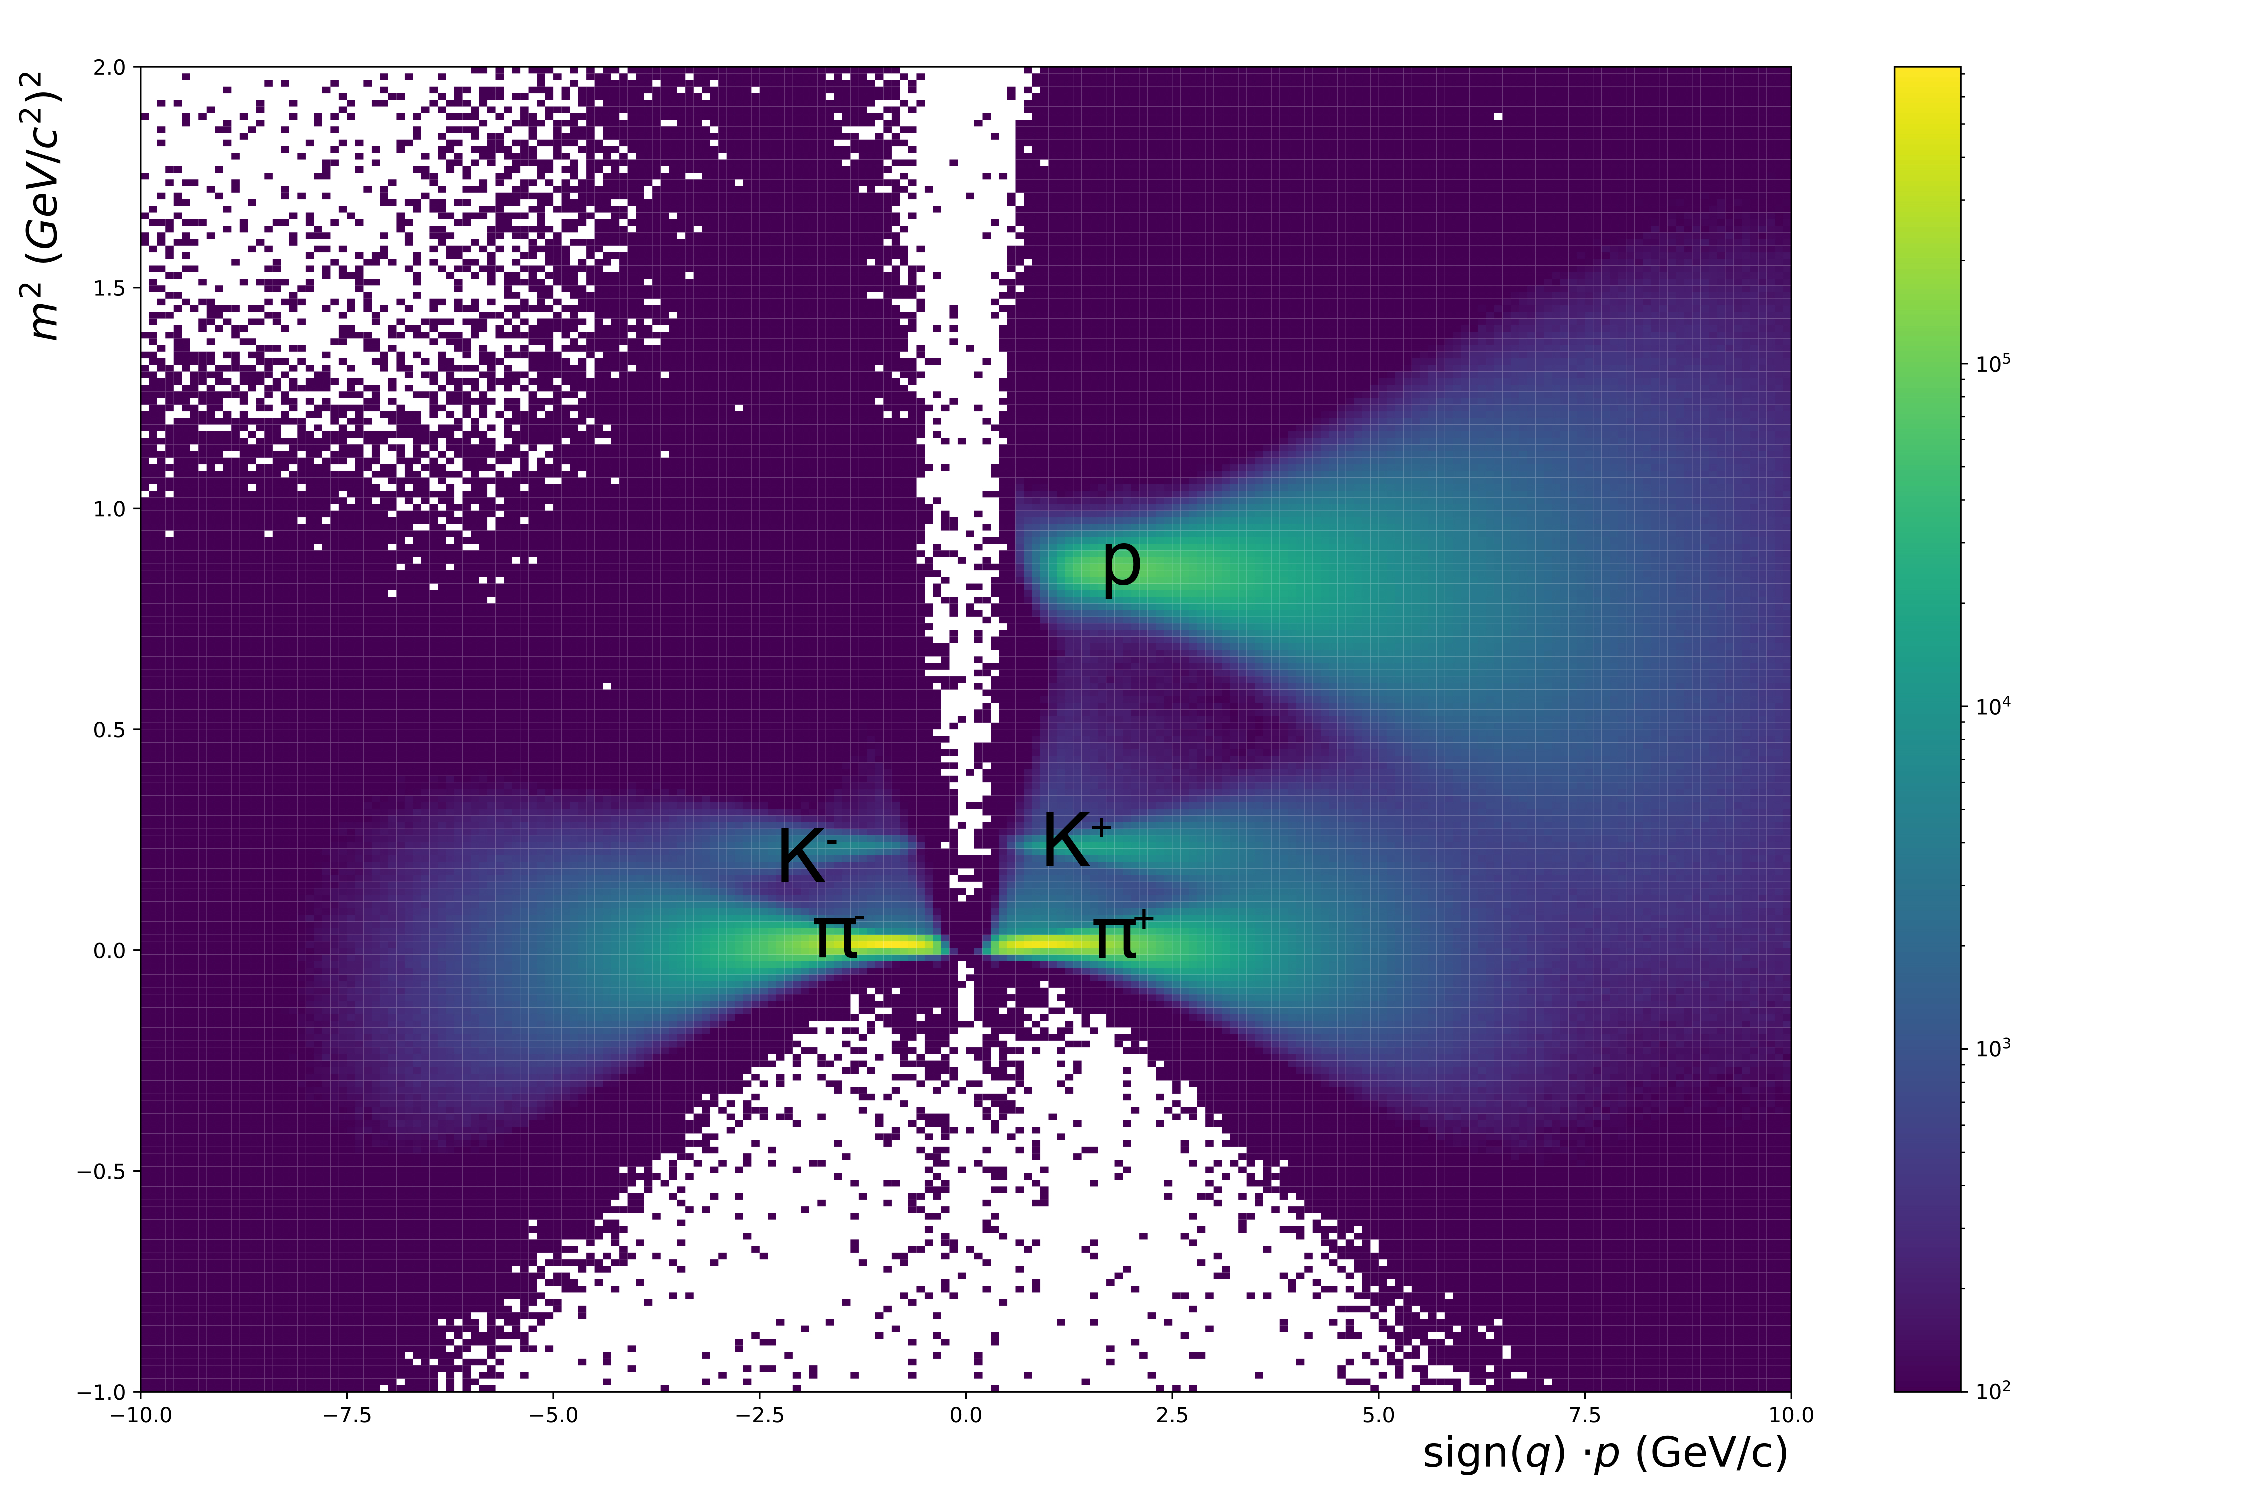
\includegraphics[width=.9\textwidth]{inz_szablon_new/img/tof_plot.pdf}
    \caption{2D TOF plot with pions, kaons, and protons shown}
    \label{tof plot}
\end{figure}
    

%%%%%%%%%%%%%%%%% KFPF
\section{Short-lived particles reconstruction}

Short-lived particles like $\Lambda^0$, and \PKshort have a neutral charge, therefore they cannot be detected directly using e.g., the TOF method. However, we can reconstruct these particles by investigating their \emph{daughter particles} - particles coming from their decays. For example, in the main decay mode (66.7\%) a K-short particle decays into a positive and negative pion (Figure \ref{ks decay}). Using i.e. the STS, we can reconstruct the tracks of pions (identified earlier using e.g., TOF method) coming from this decay, and thus reconstruct the K-short particle.

\begin{figure}[H]
\centering
    \includegraphics[width=.4\textwidth]{img/kdecay1.png}
    \caption{\PKshort main decay mode \cite{kdecay1}}
    \label{ks decay}
\end{figure}

In order to do so, the \textbf{KFParticleFinder} was developed \cite{kfp}. It is an on-line optimized particle reconstruction package based on Kalman Filter mathematics. It finds pairs of positive and negative pions (in the \PKshort case) which could be a result of the \emph{mother} particle's decay.
%------------------------- PFSimple
\subsection{PFSimple}
For offline selection optimization and analysis, \textbf{PFSimple} package was created \cite{lubynets}. Using it, one can optimize selection criteria to differentiate between:
\begin{itemize}
    \item \textbf{signal} - pion pairs created in K-short decay
    \item \textbf{background} - pions pairs returned by KFParticleFinder which are not the result of K-short decay
\end{itemize}
Also, PFSimple returns these attributes of each reconstructed particle (visualised on Figure \ref{pfsimple}):
\begin{itemize}
    \item \textbf{L/$\Delta$L} - distance between primary and secondary vertex divided over its error
    \item \textbf{DCA} - distance of closest approach between pion tracks
    \item \textbf{$\chi^2$ geo} - dimensionless distance of closest approach between pion tracks
    \item \textbf{$\chi^2$ topo} - dimensionless distance of closest approach between extrapolated kaon trajectory and primary vertex
    \item \textbf{$\chi^2$ prim} - dimensionless distance between extrapolated secondary track and primary vertex
    \item \textbf{$\cos(\alpha)$} - cosine of angle between pion and K-short momenta
\end{itemize}
\begin{figure}[H]
    \centering
    \includegraphics[width=.9\textwidth]{img/pfsimple_variables.png}
    \caption{Decay scheme and topological variables of a \PKshort decay in the PFSimple}
    \label{pfsimple}
\end{figure}
%------------------------- optimization of selection criteria
\subsubsection{Optimization of selection criteria}
As the KFParticle Finder (and PFSimple) return all the possible pion pairs, which could be a result of K-short decay,  some selection criteria need to be applied to differentiate between the signal and background.\\

The manual selection criteria can also be visualised with a decision tree (Figure \ref{manual tree}):
\begin{itemize}
    \item For each variable of a reconstructed particle, a conditional statement is being set
    \item If all conditions are fulfilled, a K-short candidate is treated as a signal  candidate
\end{itemize}

\begin{figure}[H]
    \centering
    \includegraphics[width=.6\textwidth]{img/decision_tree.png}
    \caption{Example of a decision tree using manual selection criteria}
    \label{manual tree}
\end{figure}

The manual procedure for selection criteria optimization \cite{lubynets} is as follows:
\begin{enumerate}
    \item The goal is to suppress as much background and to preserve as much signal as possible 
    \item Plot distribution of signal and background for some variable (e.g., on Figure \ref{manual distributions}), and select a point above which all entries are considered as signal or background
    \item Repeat it for all the variables
\end{enumerate}
\begin{figure}[H]
    \centering
    \includegraphics[width=1\textwidth]{img/pfsimple_distributions.pdf}
     \caption{Example of distributions to be checked with the manual selection criteria optimization}
     \label{manual distributions}
\end{figure}

However, this task is non-automatized (must be repeated for each particle), collision simulating model dependent, and only linear (as one variable at a time is used). In this work, the application of ML algorithm for the optimization of selection criteria will be discussed.

\chapter{Optimizing \PKshort reconstruction using ML}
\pagestyle{fancy}
%%%%%%%%%%%%%%%%% KOS reconstruction

In this chapter, the application of the ML algorithms for the optimization of selection criteria for \PKshort reconstruction (and thus proper identification) will be discussed. As opposed to the traditional method of optimization of selection criteria, mentioned in the chapter before, the predicted advantages and disadvantages are presented in Table \ref{tab:mlselection}.
\begin{table}[H]
    \begin{tabular}{|l|l}
    \hline
    \multicolumn{1}{|c|}{\textbf{Advantages}}        & \multicolumn{1}{c|}{\textbf{Disadvantages}}    \\ \hline
    Non-linear in multi-dimensional space            & \multicolumn{1}{l|}{Not easily interpretable}  \\ \hline
    Automatization of the selection process          & \multicolumn{1}{l|}{Computationally expensive} \\ \hline
    Partially collision simulating model-independent &                                                \\ \cline{1-1}
    \begin{tabular}[c]{@{}l@{}}With \emph{probability} a  value from which we consider \\a particle as a K-short particle can be chosen;\\ it can aim for better reconstruction efficiency \\ or a better background reduction\end{tabular} &
       \\ \cline{1-1}
    \end{tabular}
    
\caption{\label{tab:mlselection}Advantages and disadvantages of ML selection criteria optimization}
\end{table}
\\The accuracy of these predictions will be checked in this chapter. The results of the K-short reconstruction optimization have been presented before in \cite{get involved} (some fragments of this report will be presented in the following sections).

\section{Model preparation}\thispagestyle{fancy}
The CBM collaboration stores its analysis data in a storage efficient format called an AnalysisTree. For this analysis, it is later passed through the PFSimple (C++ with ROOT framework),  which combines positive and negative pions tracks (possible K-short's daughter particles pairs) and returns variables associated with these tracks, from which we could reconstruct a K-short particle. All the possible pairs along with the variables (described in the chapter before) are available for training in the \emph{PlainTree} format, which can be loaded into Pandas Dataframe (Python), using a function prepared by the CBM-ML group \cite{plaintree}\cite{uproot}. Version 3.7 of Python was used, with the following libraries:
\begin{itemize}
    \item pandas (version 1.3.4)
    \item xgboost (version 1.3.3)
    \item scikit-learn (version 1.0.1)
    \item bayesian-optimization (version 1.1.0)
\end{itemize}
A part of the code used for the ML model training is shown in Appendix A.

\subsection{Data enriching}
There are two problems to tackle before providing datasets to our ML model: underrepresentation and dependence of collision simulation model.

%---------------dependence of collision simulation model
\subsubsection{Dependence of collision simulation model}
To make the ML model partially independent of the collision simulation model,  select:
\begin{itemize}
    \item primary Ks candidates only in 5$\sigma$ region: $0.43485 - 0.56135$ (GeV/$c^2$) from DCM-QGSM-SMM model, (simulation data)
    \item background outside 5$\sigma$ region from UrQMD model, which mimics experimental data (will be replaced by real experimental data while CBM experiment starts)
\end{itemize}
 The selection process is shown on Figure \ref{enriching}. Also, the UrQMD model is being used as a test dataset (as the model does not "know" the signal candidates from this MC model).
\begin{figure}[H]
    \centering
    \includegraphics[width=.8\textwidth]{img/dataset.png}
    \caption{Data enriching}
    \label{enriching}
\end{figure}
In total, the following datasets will be used:
\begin{itemize}
    \item 5M (2.352M) events for signal generated in DCM-QGSM-SMM
    \item 30k(50k) events for both background and test dataset generated in UrQMD
\end{itemize}
Au-Au @12A(3.3A) GeV/c passed through CBM setup in GEANT4, and PFSimple.


%---------------underrepresentation
\subsubsection{Underrepresentation}
As in the simulated data, less than 0.1\% of K-short candidates are signal candidates, the ratio in the training dataset has to be changed so that the model learns how to identify signal candidates well. Using the trail and error method, it is decided that the number of background entries is rescaled by this formula:
\begin{equation}
    n_\text{events(background)} = 5 \cdot n_\text{events(signal)}
\end{equation}


%------------- data cleaning
\subsection{Data cleaning}
To reject the numeric values of parameters that do not have physical sense, but are present in the data set, some selection criteria are applied before the beginning of the model training. Similarly, some values which might be possible but their uncertainties are big are rejected, to reduce the amount of data.

%----------------------- Invariant mass
\subsubsection{Invariant mass}
As the K-short particle decays into two pions, its invariant mass cannot be smaller than the mass of the two pions, so:
\begin{center}
    $m_\text{inv} >$ 0.279 GeV/$c^2$
\end{center}
Also, to reduce the amount of data:
\begin{center}
   $m_\text{inv} <$ 1 GeV/$c^2$
\end{center}

%---------------- distances
\subsubsection{Distances and \emph{x, y, z} coordinates}
Distance between the primary vertex (the point where the collision of the nuclei happens), and the secondary vertex (the extrapolated point where the two daughter particles should have crossed each other)  - $l$ and the distance of closest approach between the two pions - $DCA$ -  cannot be smaller than zero:
\begin{center}
    $DCA$, $l$, $\frac{l}{\Delta l}$ $> 0$
\end{center}

Also, due to the sizes of the tracking system (the largest station has an area of 1m$^2$):
\begin{center}
    $DCA < 100 $ cm
\end{center}
For the same reason:
\begin{center}
    $|x|, |y| < 50$ cm
\end{center}
As the particle has to hit 3 stations of the tracking system, and the last two are placed above 80 cm:
\begin{center}
    $l < 80$cm
\end{center}
For the same reason, and because of the fixed target geometry of the detector:
\begin{center}
    $-1$ cm $< z < 80$ cm
\end{center}
To reduce the data, we set:
\begin{center}
    $\frac{l}{\Delta l} < 15000$
\end{center}
However, in the KFParticle package $l$ is assumed to be signed by design, and one can notice that actually, some data entries have a negative value of distance, for both signal and background. As the \emph{quality cuts} should be rather conservative, the following ranges are set:
\begin{center}
     $l >$ -5 (cm)\\
     $\frac{l}{\Delta l} >$ -25
\end{center}
%----------------- momentums
\subsubsection{Momentums}
The fixed target geometry of the detector requires that:
\begin{center}
    $p_Z > 0 $ GeV/c
\end{center}
To reduce the data:
\begin{center}
    $p < 20$ GeV/c; $p_T < 3$ GeV/c
\end{center}


%-------------- chi square
\subsubsection{Chi square}
Since $\chi^2$ is a squared distance, all the values must be larger than zero:
\begin{center}
    $\chi^2 > 0$
\end{center}
To reduce the data, following the maximal values are selected:
\begin{itemize}
    \item $\chi^2$ first and second $< 3 \cdot 10^7$
    \item $\chi^2_{geo} < 10000$
    \item $\chi^2_{topo} < 100000$
\end{itemize}

%----------------------- pseudorapidity
\subsubsection{Pseudorapidity}
Pseudorapidity in terms of the polar angle can be defined as:
\begin{equation}
    \eta = -\ln{\tan(\frac{\theta}{2})}
\end{equation}
where $\theta$ - polar angle, and the STS covers the polar angles between 2.5$^{\circ}$ and 25$^{\circ}$, for which the pseudorapidity values would equal:
\begin{center}
    $ 1.5< \eta < 3.82 $
\end{center}
However, due to the magnetic field, the pseudorapidity is constrained to the following values:
\begin{center}
    $ 1.0< \eta < 6.5 $
\end{center}
with which 0.06\% of data for signal is lost (instead of 5.66\%) and 0.08\% of data for background (instead of 6.75\%)

%------------------ variables selection
\subsection{Variables selection}
The last step before training our model is the selection of variables that will be used in the training of the discriminator. To make the model simpler, there is no need to use multiple variables if they are strongly correlated with each other. Also, to avoid signal/background classification directly by invariant mass, variables strongly correlated with the invariant mass of background should be omitted.
\subsubsection{Correlation matrix}
The Pearson correlation coefficient (which shows linear correlation) of each variable is being calculated following this formula:
\begin{equation}
    \rho = \frac{\operatorname{COV}(X, Y)}{\sigma_X \times \sigma_Y}
    \label{pearson}
\end{equation}
where:
\begin{equation}
    \operatorname{COV(X, Y)} = \operatorname{E}\left[\left(X - \operatorname{E}\left[X\right]\right) \left(Y - \operatorname{E}\left[Y\right]\right)\right]
\end{equation}
\begin{equation}
    \sigma_X = \sqrt{\operatorname{E}\left[\left(X - \operatorname{E}\left[X\right]\right)^2\right]}
    \label{stddev}
\end{equation}
They are then plotted in a matrix shown on Figure \ref{correlation matrix} (where chi2... means $\chi^2$..., distance - $DCA$, loverdl - $\frac{l}{\Delta l}$). For example  e, it shows that there is no need to use  \emph{rapidity}, $p$, $p_T$ and $p_z$ for training, as those four variables are highly correlated ($\rho > 0.5$). 
\begin{figure}[h!]
    \centering
    \includegraphics[width=1.1\textwidth]{img/Correlations_of_all_variables_for_both_background_and_signal_after_quality_cuts_(pearson).pdf}
    \caption{Correlation matrix}
    \label{correlation matrix}
\end{figure}
\clearpage
%-------------------- Correlation with invariant mass
\subsubsection{Correlation with invariant mass}
The correlation (Pearson coefficient) of each variable with the invariant mass of (separately) signal and background is being checked (plotted on Figure \ref{all variables}).
\begin{figure}[H]
    \centering
    \includegraphics[width=1\textwidth]{img/Correlation_of_all_variables_with_mass_along_with_SEM.pdf}
    \caption{Correlation of all variables with mass}
    \label{all variables}
\end{figure}

%-------------------- Selected variables
\subsubsection{Selected variables}
Based on that, the following 6 variables are selected for the training: $L/\Delta L$, $DCA$;  $\chi^2_{geo}$, $\chi^2_{topo}$, $\chi^2_{prim first}$, $\chi^2_{prim second}$

%----------------------- Model training
\section{Model training}
The model will be trained and tested differently on two collision energies of the CBM experiment: $p_{\text{beam}}$ = 12A GeV/c (described in the first subsection) and $p_{\text{beam}}$ = 3.3A GeV/c (described in the second subsection).
%--------- results for 12A GeV/c
\subsection{Results for $p_{\text{beam}}$ = 12A GeV/c}
Having prepared the data, the training of the ML algorithm may be initiated. To choose the hyper-parameters values of the XGBoost model, the Bayesian Optimisation package was used.  Along with splitting the train dataset into two equal parts: one for actual training, and the second for validation, the aim is to omit overfitting of the model on the training data. \\
%--------------- Cross validation
\subsubsection{Validation on test dataset}
To check if the model works as well on the test data, as on the training dataset,  Receiver Operating Characteristic (Figure \ref{ROC}) and probability plots (Figure \ref{Probability plot}) are drawn.

Receiver Operating Characteristic illustrates the diagnostic ability of a binary classifier. Threshold on the ROC (Receiver Operating Characteristic) curve which maximizes Approximate Median Significance 
\begin{equation}
    \text{AMS}= \sqrt{2} [(tpr + fpr) \log(1 + tpr/fpr) - tpr]
\end{equation}
(where $t(f)pr$ is true (false) positive rate) on the test sample is the best threshold.
\begin{figure}[H]
    \centering
    \includegraphics[width=.98\textwidth]{img/ams.pdf}
    \caption{Receiver Operating Characteristic}
    \label{ROC}
\end{figure}
We see that the optimal point on ROC is similar for both train and test datasets.
Based on signal/background share in both train and test datasets from the probability plot (Figure \ref{Probability plot}), it is observed that the results are similar for the two datasets. Hence, we can say that our model is not overtrained (works well on new data).
\begin{figure}[H]
    \centering
    \includegraphics[width=.8\textwidth]{img/probability.pdf}
    \caption{Probability plot}
    \label{Probability plot}
\end{figure}

The invariant mass distribution before and after XGB selection is presented on Figure \ref{Invariant mass distribution}:
\begin{figure}[h!]
    \centering
    \includegraphics[width=.88\textwidth]{img/cut_visualization.png}
    \caption{Invariant mass distribution}
    \label{Invariant mass distribution}
\end{figure}


%--------------- Comparison with default KFPF Cuts
\subsubsection{Comparison with default KFPF Cuts}
KFParticleFinder has default selection criteria, which can be compared with ML selection:
\begin{itemize}
    \item $L/\Delta L > 5 $
    \item $DCA < 1 $ cm
    \item $\chi^2_{geo} < 3 $
    \item $\chi^2_{prim} > 18.4 $
    \item $\cos(\alpha) > 0 $
\end{itemize}
Depending on the cut value,  better background reduction or better efficiency can be obtained.

With a cut value set to 0.99, we get $50\times$ less background (Fig. \ref{bckgr}):
\begin{itemize}
    \item \textbf{Reconstructed \PKshort / reconstructible \PKshort = 80.67\%}  vs. 76.93\% with default KFPF cuts
    \item \textbf{false / true positive rate = 0.04} vs. 2.01 with default KFPF cuts
\end{itemize}
\begin{figure}
 \centering
    \begin{subfigure}[b]{0.99\linewidth} 
        \centering
        \includegraphics[width=\textwidth]{img/better_reduction1.png} 
        \caption{Invariant mass distribution (y log scale)} 
        \vspace{0.3cm}
    \end{subfigure}
     \hfill
       \begin{subfigure}[b]{0.99\linewidth}
        \centering
        \includegraphics[width=\textwidth]{img/better_reduction2.png} 
        \caption{Invariant mass distribution (close-up)}
        \vspace{0.3cm}
    \end{subfigure}
    \caption{Comparison with KFPF cuts}\label{bckgr}
\end{figure}

With a cut value set to 0.86, we get $20\%$ better efficiency (Fig. \ref{effic}):
\begin{itemize}
    \item \textbf{Reconstructed \PKshort / reconstructible \PKshort = 95.91\%}  vs. 76.93\% with default KFPF cuts
    \item \textbf{false / true positive rate = 1.27} vs. 2.01 with default KFPF cuts
\end{itemize}
\begin{figure}
 \centering
    \begin{subfigure}[b]{0.99\linewidth} 
        \centering
        \includegraphics[width=\textwidth]{img/better_efficiency1.png} 
        \caption{Invariant mass distribution (y log scale)} 
        \vspace{0.3cm}
    \end{subfigure}
     \hfill
       \begin{subfigure}[b]{0.99\linewidth}
        \centering
        \includegraphics[width=\textwidth]{img/better_efficiency2.png} 
        \caption{Invariant mass distribution (close-up) - comparison with KFPF cuts}
        \vspace{0.3cm}
    \end{subfigure}
    \caption{Invariant mass distribution for probability $>$ 0.86}\label{effic}
\end{figure}

%--------------------- Investigation of potential bias
\subsubsection{Investigation of potential bias}
To check if the XGB selection criteria cut tails of the distribution, or are biased in some regions, the invariant mass distribution of true and false positives is plotted (Figure. \ref{true-false}).
\begin{figure}[h!]
 \centering
    \begin{subfigure}[b]{0.79\linewidth} 
        \centering
        \includegraphics[width=\textwidth]{img/true_and_false_signal.png} 
        \caption{Selected \PKshort and false positives distribution} 
        \vspace{0.3cm}
    \end{subfigure}
     \hfill
       \begin{subfigure}[b]{0.69\linewidth}
        \centering
        \includegraphics[width=\textwidth]{img/efficiency_plot_mass.png} 
        \caption{Reconstructed and MC true positives (y log scale)}
        \vspace{0.3cm}
    \end{subfigure}
    \caption{True-false positives investigation}
    \label{true-false}
\end{figure}
We see that our model does not seem to be biased towards any invariant mass region.

\newpage
%----------------------- results for 3.3A GeV/c
\subsection{Results for $p_{\text{beam}}$ = 3.3A GeV/c}

\subsubsection{Comparison with KFPF cuts}
The same code can be used to obtain similar results for another CBM energy level. Comparing to default KFPF cuts, with probability cut 0.9635 (Fig. \ref{33agev}):
\begin{itemize}
    \item \textbf{Reconstructed \PKshort / reconstructible \PKshort = 93.45\%}  vs. 78.94\% with default KFPF cuts
    \item \textbf{false / true positive rate = 0.19} vs. 1.38 with default KFPF cuts
\end{itemize}

\begin{figure}[h!]
 \centering
    \begin{subfigure}[b]{0.99\linewidth} 
        \centering
        \includegraphics[width=\textwidth]{img/kaon_inv_mass_comparison_closeup.pdf} 
        \caption{Invariant mass distribution (y log scale)} 
        \vspace{0.3cm}
    \end{subfigure}
     \hfill
       \begin{subfigure}[b]{0.99\linewidth}
        \centering
        \includegraphics[width=\textwidth]{img/circle_kshort_invmass_with_ML.png} 
        \caption{Invariant mass distribution (close-up)}
        \vspace{0.3cm}
    \end{subfigure}
    \caption{Comparison with KFPF cuts for 3.3A GeV/c}\label{33agev}
\end{figure}
Due to the smaller statistics for this energy level, the ML model training should be redone for a bigger dataset.

%-------------- Influence of the magnetic field scaling
\subsection{Influence of the magnetic field scaling}
Obtained ML model can be adapted for the investigation of the influence of the magnetic field scaling. We compare: 100\% MF strength (for  $p_{\text{beam}}$ = 12A GeV/c), 56\% and 27.5\% MF strength (for $p_{\text{beam}}$ = 3.3A GeV/c, both with only DCM generated data for 0.4M events for training and 0.1M for validation). We see (Fig. \ref{mf}) that the stronger the magnetic field is, the broader \PKshort invariant mass distribution peak is. Also, we observe much more signal entries for $p_{\text{beam}}$ = 12A GeV/c (for the same number of events). \\

For $p_{\text{beam}}$ = 3.3A GeV/c the number of signal entries is almost the same; we select the probability cut so that the false/true positive ratio is the same for both \% of MF and compare the efficiency of the reconstruction (Tab. \ref{tab:mf}). We see that weaker MF does not necessarily worsen efficiency (only 2\% difference). However, this comparison should also be redone for a bigger dataset.

\begin{table}[h!]
\begin{tabular}{|l|l|l|l|}
\hline
\textbf{ratio} &
  \textbf{\begin{tabular}[c]{@{}l@{}}12 A GeV/c \\ MF=100\%\end{tabular}} &
  \textbf{\begin{tabular}[c]{@{}l@{}}3.3 A GeV/c \\ MF=56\%\end{tabular}} &
  \textbf{\begin{tabular}[c]{@{}l@{}}3.3 A GeV/c \\ MF=27.5\%\end{tabular}} \\ \hline
\begin{tabular}[c]{@{}l@{}}reconstructed/\\ reconstructible\end{tabular} &
  89.98\% &
  90.36\% &
  88.49\% \\ \hline
\begin{tabular}[c]{@{}l@{}}false / \\ true positive\end{tabular} &
  0.2 &
  0.2 &
  0.2 \\ \hline
\end{tabular}
\caption{\label{tab:mf}Comparison of MF strength vs. efficiency}
\end{table}

\begin{figure}[h!]
 \centering
    \includegraphics[width=\textwidth]{img/mf0log.pdf} 
    \vspace{0.1cm}
    \caption{Invariant mass distribution for different MF scaling}
    \label{mf}
\end{figure}



\chapter{''TOF'' particles identification using ML}
\pagestyle{fancy}
%%%%%%%%%%%%%%%%% ML
In this chapter, the application of the ML algorithms for particles identification (as equivalent of the TOF method) will be discussed. As opposed to the traditional TOF method, instead of plotting mass-squared and $p \cdot q$, and then fitting gaussians to the distributions to differentiate between the particles group, the data from MVD+STS and TOF detectors will be provided directly to the ML model. The aim is to differentiate between the three groups of particles:
\begin{itemize}
    \item protons
    \item kaons
    \item pions (in the third group, the muons and electrons are included as well, as their mass-squared is almost indistinguishable without the data from other detectors)
\end{itemize}
\begin{figure}[h!]
    \centering
    \includegraphics[width=.8\textwidth]{inz_szablon_new/img/m2tof.pdf}
    \caption{Histograms of mass-squared of each particle class (differences of quantity of each particle type can also be observed)}
\end{figure}

%-------------------------Model preperation
\section{Model preparation}\thispagestyle{fancy}
In this chapter, the data from the detectors saved in the AnalysisTree format is converted into a PlainTree format using a C++ program with ROOT libraries. Its fragments are presented in the appendix B. The following variables can be used:
\begin{itemize}
    \item From MVD+STS: charge sign ($q$); momentum components: $p, p_T, p_x, p_y, p_z$; rapidity and pseudorapidity ($\eta$); azimuthal angle ($\phi$)
    \item From TOF: mass-squared ($m^2$), calculated by formula \ref{msquared} (using $p$ value from MVD+STS)
    \item From MC model: invariant mass; PID code, which returns the information about the type of particle in the PDG convention, e.g., -2212 = (-)anti—(2212)proton\cite{hepnames}
\end{itemize}
The same libraries were used as in the chapter 6. For training and validation, the following datasets are used:
\begin{itemize}
    \item 2M events generated in DCM-QGSM-SMM (training dataset)
    \item 1M events generated in UrQMD (test dataset)
\end{itemize}
Au-Au @12A GeV/c passed through CBM setup in GEANT4, and PFSimple. The different models used for training and validation allow us to check, if the ML model is not biased towards a specific MC model. 
%----------------------Data enriching
\subsection{Data enriching}
%------------Renaming
\subsubsection{Remapping}
The four different classes will be loaded into the ML model:
\begin{itemize}
    \item 0: protons
    \item 1: kaons
    \item 2: pions (with the muons and electrons)
    \item 3: \emph{background} - all the other particles
\end{itemize}
The classes 0-2 are loaded into the model during the training. Later, if the probability returned by the XGB is smaller than a specific threshold, the particle is identified as 3 - background.
%------------Underrepresentation
\subsubsection{Underrepresentation}
As different classes have different number of particles, they are rescaled so that each class has the same number of elements (in this case, it is specified by the number of Kaons, as they are the most underrepresented class).
%-------------------------Data cleaning
\subsection{Data cleaning}
To reject the numeric values of parameters which do not have physical sense, but are present in the data set, some selection criteria are applied before the beginning of the model training. Similarly to the chapter 6, we some values which might be possible but are rare enough are rejected, to reduce the amount of data.

%----------------------- Invariant mass
\subsubsection{Mass-squared}
To constraint the mass-squared region to the one of the selected classes:
\begin{center}
    -1 $ < m^2 < $ 2 $(GeV/c^2)^2$
\end{center}
Later during the training (not for the validation dataset), the mass-squared of each class will be constrained to a specific value of $\sigma$ - standard deviation (\ref{stddev}) around its mean value. After some tests, the following values were chosen: $1 \sigma$ region for ID=0 and ID=2; $1.5 \sigma$ for kaons (ID=1)
\begin{figure}[H]
    \centering
    \includegraphics[width=.8\textwidth]{inz_szablon_new/img/all_particles_b.pdf}
    \caption{2D TOF histogram of all particles after data cleaning}
\end{figure}
\begin{figure}[H]
    \centering
    \includegraphics[width=.8\textwidth]{inz_szablon_new/img/TOF 2D plot for all simulated particle ID = 0.pdf}
    \caption{2D TOF histogram of protons (ID=0) after $1 \sigma$ selection}
\end{figure}
\begin{figure}[H]
    \centering
    \includegraphics[width=.8\textwidth]{inz_szablon_new/img/TOF 2D plot for all simulated particle ID = 1.pdf}
    \caption{2D TOF histogram of kaons (ID=1) after $1.5 \sigma$ selection}
\end{figure}
\begin{figure}[H]
    \centering
    \includegraphics[width=.8\textwidth]{inz_szablon_new/img/TOF 2D plot for all simulated particle ID = 2.pdf}
    \caption{2D TOF histogram of pions, muons and electrons (ID=2) after $1 \sigma$ selection}
\end{figure}
%----------------- momentums
\subsubsection{Momentums}
The fixed target geometry of the detector requires that:
\begin{center}
    $p_Z > 0 $ GeV/c
\end{center}
To reduce the data:
\begin{center}
    $p < 12$ GeV/c; $p_T < 2$ GeV/c
\end{center}
%--------------- variables selection
\subsection{Variables selection}
In this chapter, the TOF identification method is recreating, so the $m^2$, $p$ and $q$ values are being used. However, the results coming from only those 2 values were not perfect (usually, it is better to train a XGBoost model using multiple variables). After plotting the correlation matrix (Figure \ref{cmatrix tof}), and following the other works\cite{ostrowski}, the $p_T$ and $\eta$ values are being selected also. 

\begin{figure}[h!]
    \centering
    \includegraphics[width=1.1\textwidth]{inz_szablon_new/img/Correlations_TOF.pdf}
    \caption{Correlation matrix}
    \label{cmatrix tof}
\end{figure}

%---------------------Model training
\section{Model training}
With the prepared data, the ML model training can be started. Once again, the hyperparameters are being selected using Bayesian Optimisation. 

%%%%%%%------------- Probability cuts
\subsection{Probability plots}
This time (contrary to K-short reconstruction optimisation), our model is a multi-class classifier (non-binary). For each particle, it returns the probability of belonging to each (0-2) class. The probability plot for all the classes can be plotted:
\begin{figure}[H]
    \centering
    \includegraphics[width=.9\textwidth]{inz_szablon_new/img/proba_before_cut .pdf}
    \caption{Probabilities distribution for all the classes}
\end{figure}

Later, the probability plot for each class can also be made, showing probability for all the particle vs. true-positives (particles belonging to the class). It allows to set a certain threshold, below which it is better to classify a particle as background (ID=3). With this approach, the number of false-positives is smaller; it also includes particles which don't belong to the 0-2 classes (e.g., $\Sigma^\pm$):
\begin{figure}[H]
    \centering
    \includegraphics[width=.88\textwidth]{inz_szablon_new/img/proba_protons .pdf}
    \caption{Probability distribution for ID=0 }
\end{figure}
\begin{figure}[H]
    \centering
    \includegraphics[width=.88\textwidth]{inz_szablon_new/img/proba_kaons .pdf}
    \caption{Probability distribution for ID=1}
\end{figure}
\begin{figure}[H]
    \centering
    \includegraphics[width=.88\textwidth]{inz_szablon_new/img/proba_pions .pdf}
    \caption{Probability distribution for ID=2 }
\end{figure}
The following thresholds (which aim for as big efficiency as possible, with correct shape of mass-squared distribution (plotted later)): were decided:
\begin{itemize}
    \item for ID = 0 : 0.88
    \item for ID = 1 : 0.96
    \item for ID = 2 : 0.82
\end{itemize}

%%%%%%%------------- Confusion matrix
\subsection{Confusion matrix}
Confusion matrix is useful in checking the accuracy of a classifier. By definition a confusion matrix $C$ is such that $C_{i, j}$ is equal to the number of observations known to be in group $i$ and predicted to be in group $j$. Thus in binary classification, the count of true negatives is $C_{0, 0}$, false negatives is $C_{1, 0}$, true positives is $C_{1, 1}$  and false positives is $C_{0, 1}$\cite{cmatrix}. Normalized confusion matrix shows not the number of observations for each class, but the percentage.

For our model, the confusion matrices after applying the probability threshold are plotted on Figures \ref{cm} and \ref{cm_norm}.

Using the information from the confusion matrix, the efficiency of classifier can be put in the Table \ref{tab:tof}.

\begin{figure}[h!]
    \centering
    \includegraphics[width=1\textwidth]{inz_szablon_new/img/cm.pdf}
    \caption{Confusion matrix}
    \label{cm}
\end{figure}
\begin{figure}[h!]
    \centering
    \includegraphics[width=1\textwidth]{inz_szablon_new/img/cm_norm.pdf}
    \caption{Confusion matrix (normalised)}
    \label{cm_norm}
\end{figure}



\begin{table}[h!]
    \begin{tabular}{|c|c|c|c|}
    \hline
    \textbf{ID} & \textbf{Efficiency} & \textbf{Efficiency of true positives} & \textbf{False/True ratio} \\ \hline
    \textbf{0} & 108\% & 92.88\% & 0.17 \\ \hline
    \textbf{1} & 119\% & 72.48\% & 0.65 \\ \hline
    \textbf{2} & 102\% & 91.60   & 0.12 \\ \hline
    \end{tabular}
\caption{\label{tab:tof}Efficiency of the ML model for TOF identification}
\end{table}

%--------------- Mass-squared distributions
\subsection{Mass-squared distributions}
After the ML model training and running it on the test dataset, the following invariant mass distributions are returned by it:

\begin{figure}[h!]
    \centering
    \includegraphics[width=.8\textwidth]{inz_szablon_new/img/m20.pdf}
    \caption{Mass-squared distributions for particles ID = 0}
\end{figure}
\begin{figure}[h!]
    \centering
    \includegraphics[width=.8\textwidth]{inz_szablon_new/img/m21.pdf}
    \caption{Mass-squared distributions for particles ID = 1}
\end{figure}
\begin{figure}[h!]
    \centering
    \includegraphics[width=.8\textwidth]{inz_szablon_new/img/m22.pdf}
    \caption{Mass-squared distributions for particles ID = 2}
\end{figure}

%----------------------Analysis of the results
\section{Analysis of the results}
While the mass-squared distributions are useful, simple visualisation of the classifier results, the TOF plots are more handy in analyzing the way the ML model works. The XGBoost-selected partic;es can be plotted with the simulated particles (all the particles that should be reconstructed) for each class.

\subsubsection{ID = 0 (protons)}
For particles ID = 0 (protons) we observe, that the protons of mass-squared close to 0 (mostly protons coming directly from the bullet particle) are not identified correctly. Hovewer, they should be treated as a different class, as the sigma-selection cuts them out during the training. For the same reason protons with high $p$, but small mass-squared are not identified at all.
\begin{figure}[H]
 \centering
    \begin{subfigure}[b]{0.7\linewidth} 
        \centering
        \includegraphics[width=\textwidth]{inz_szablon_new/img/xgb 0.pdf}
        \caption{XGBoost selected particles}
        \vspace{0.3cm}
    \end{subfigure}
     \hfill
       \begin{subfigure}[b]{0.7\linewidth}
        \centering
        \includegraphics[width=\textwidth]{inz_szablon_new/img/sim 0.pdf}
        \caption{Simuated particles}
        \vspace{0.3cm}
    \end{subfigure}
    \caption{2D TOF plot for ID = 0}
\end{figure}
\clearpage

\subsubsection{ID = 1 (kaons)}
For particles ID = 1 (kaons) the efficiency, and the false-positive ratio are the most deviated from the correctness. The ML model with the high value of the threshold chosen picks only kaons with small $p$ value. Also, one region of kaons close to $m^2 = 2$ is also not used in training - however, it may be a result of a mismatch in the simulation, as the kaons are not expected in this region.
\begin{figure}[H]
 \centering
    \begin{subfigure}[b]{0.7\linewidth} 
        \centering
        \includegraphics[width=\textwidth]{inz_szablon_new/img/xgb 1.pdf}
        \caption{XGBoost selected particles}
        \vspace{0.3cm}
    \end{subfigure}
     \hfill
       \begin{subfigure}[b]{0.7\linewidth}
        \centering
        \includegraphics[width=\textwidth]{inz_szablon_new/img/sim 1.pdf}
        \caption{Simuated particles}
        \vspace{0.3cm}
    \end{subfigure}
    \caption{2D TOF plot for ID = 1}
\end{figure}
\clearpage

\subsubsection{ID = 2 (pions, muons and electrons)}
For particles ID = 2 (pions, muons and electrons) have the best efficiency, as most of the particles of the lowers mass-squared values belong to one of these classes. Once again there is a region that is not expected - electrons of $m^2 \approx 2$, which are mostly probably a result of the mismatch in the simulation of the CBM setup.
\begin{figure}[H]
 \centering
    \begin{subfigure}[b]{0.7\linewidth} 
        \centering
        \includegraphics[width=\textwidth]{inz_szablon_new/img/xgb 2.pdf}
        \caption{XGBoost selected particles}
        \vspace{0.3cm}
    \end{subfigure}
     \hfill
       \begin{subfigure}[b]{0.7\linewidth}
        \centering
        \includegraphics[width=\textwidth]{inz_szablon_new/img/sim 2.pdf}
        \caption{Simuated particles}
        \vspace{0.3cm}
    \end{subfigure}
    \caption{2D TOF plot for ID = 2}
\end{figure}
\clearpage

\subsubsection{ID = 3 (background)}
Particles ID = 3 (background) was mostly assigned to the particles of mass-squared close to the value of the mean mass-squared of kaons, but with bigger $p$ values. It can also be seen in the confusion matrix - 0.14\% of kaons are misidentified as background, as well as kaons and ID = 2 particles which, were found in this $m^2$ region.
\begin{figure}[H]
 \centering
    \begin{subfigure}[b]{0.7\linewidth} 
        \centering
        \includegraphics[width=\textwidth]{inz_szablon_new/img/xgb 3.pdf}
        \caption{XGBoost selected particles}
        \vspace{0.3cm}
    \end{subfigure}
     \hfill
       \begin{subfigure}[b]{0.7\linewidth}
        \centering
        \includegraphics[width=\textwidth]{inz_szablon_new/img/sim 3.pdf}
        \caption{Simuated particles}
        \vspace{0.3cm}
    \end{subfigure}
    \caption{2D TOF plot for ID = 3}
\end{figure}
\clearpage
\chapter{Discussion and summary}


mogło być źle, ale będzie lepiej
\chapter{Appendix A}
\pagestyle{fancy}
\thispagestyle{fancy}
Kod rekontrukcja kaonow ML
\chapter{Appendix B}
\pagestyle{fancy}
\thispagestyle{fancy}

Framgents of code (\emph{ATreePlainer.cpp}) class used for transforming data in AnalysisTree format into PlainTrees, ready for loading into Pandas Dataframe is presented here.

\lstset{language=C++}
\begin{lstlisting}
#include "ATreePlainer.hpp"
#include "AnalysisTree/TaskManager.hpp"

//Initializes variables associated with each AnalysisTree Branch
void ATreePlainer::Init()
{
  //Initating AnalysisTree Task Manager
  auto* man = AnalysisTree::TaskManager::GetInstance();
  auto* chain = man->GetChain();

  //Variables for each AnalysisTree branch
  tofhits_ = ANALYSISTREE_UTILS_GET<AnalysisTree::
    Detector<AnalysisTree::Hit>*>(chain->GetPointerToBranch("TofHits"));
  simulated_= ANALYSISTREE_UTILS_GET<AnalysisTree::
    Particles*>(chain->GetPointerToBranch("SimParticles"));
  tof2sim_match_ = chain->GetMatchPointers().find(config_->GetMatchName(
    "TofHits", "SimParticles"))->second;
  vtxtracks_ = ANALYSISTREE_UTILS_GET<AnalysisTree::Detector<AnalysisTree::
    Track>*>(chain->GetPointerToBranch("VtxTracks"));
  vtx2tof_match_ = chain->GetMatchPointers().find(config_->GetMatchName(
    "VtxTracks", "TofHits"))->second;

  //Initating output PlainTree
  auto out_config = AnalysisTree::TaskManager::GetInstance()->GetConfig();
  AnalysisTree::BranchConfig out_particles("Complex", AnalysisTree::
    DetType::kParticle);
  out_particles.AddField<float>("mass2");
  out_particles.AddField<int>("q");
  man->AddBranch("Complex", plain_branch_, out_particles);
  InitIndices();
}

//Transformation of AnalysisTree into PlainTree
void ATreePlainer::Exec()
{
  plain_branch_ -> ClearChannels();
  auto out_config = AnalysisTree::TaskManager::GetInstance()->GetConfig();

    //Loop over all reconstructed particles from the TOF detector
   for(auto& input_particle : *tofhits_)
   {
       const auto matched_particle_sim_id = tof2sim_match_->GetMatch(
        input_particle.GetId());
       //Matching with input from MC information about particles
       if (matched_particle_sim_id > 0){
         const auto matched_particle_vtx_id = vtx2tof_match_->GetMatchInverted(
            input_particle.GetId());
         //Matching with data from STS+MVD (VtxTracks branch)
         if (matched_particle_vtx_id > 0){
           //from tof
            auto& output_particle = plain_branch_->AddChannel(
                out_config->GetBranchConfig(plain_branch_->GetId()));
            output_particle.SetField(input_particle.GetField<float>(
                mass2_id_tof_), mass2_id_w1_);
            //from simulated
            auto& matched_particle_sim = simulated_->GetChannel(
                matched_particle_sim_id);
            output_particle.SetMass(matched_particle_sim.GetMass());
            output_particle.SetPid(matched_particle_sim.GetPid());
            //from VtxTracks
            auto& matched_particle_vtx = vtxtracks_->GetChannel(
                matched_particle_vtx_id);
            output_particle.SetMomentum3(matched_particle_vtx.GetMomentum3());
            output_particle.SetField(matched_particle_vtx.GetField<int>(
                q_id_vtx_), q_id_w1_);
            }
          }
      }
}

//Indicies for the output PlainTree
void ATreePlainer::InitIndices()
{
  //Variables from the input file, which are not defined by default
   auto in_branch_tof = config_->GetBranchConfig("TofHits");
   mass2_id_tof_     = in_branch_tof.GetFieldId("mass2");
   auto in_branch_vtx = config_->GetBranchConfig("VtxTracks");
   q_id_vtx_         = in_branch_vtx.GetFieldId("q");
  //Variables in the output file
   auto out_config = AnalysisTree::TaskManager::GetInstance()->GetConfig();
   const auto& out_branch = out_config->GetBranchConfig(
    plain_branch_->GetId());
   mass2_id_w1_           = out_branch.GetFieldId("mass2");
   q_id_w1_               = out_branch.GetFieldId("q");
}



\end{lstlisting}
\chapter{Appendix C}
\pagestyle{fancy}
\thispagestyle{fancy}

Kod identyfikacja TOF ML
\begin{thebibliography}{99}
	% Zmieniæ na 99, w przypadku, gdy bibliografia liczy wiêcej ni¿ 9 pozycji.
	% W przypadku du¿ej liczby pozycji, wygodniej korzystaæ z BibTeXa.
	% Zalecany wzór wpisu bibliograficznego dla publikacji z czasopisma: nazwiska i inicja³y imion (przy dwóch imionach bez spacji po kropce!) autorów pisane s¹ kapitalikami. Nastêpnie dwukropek i tytu³ pracy pisany kursyw¹. Nastêpnie kropka i nazwa czasopisma, volume (pogrubiony), rok i numery stron. W przypadku podawania przedzia³ów liczbowych u¿ywa siê pó³pauzy (--) bez spacji, a nie ³¹cznika (-)!
	% Zalecany wzór wpisu dla ksi¹¿ki: nazwiska i inicja³y imion kapitalikami; nastêpnie dwukropek i tytu³ kursyw¹. Po kropce numer wydania (opcjonalnie), nazwa wydawnictwa, miejsce i rok wydania.
	\thispagestyle{fancy}
	\bibitem{zbroszczyk} Hanna Paulina Zbroszczyk. ''Eksperymentalne aspekty badania korelacji femtoskopowych w zderzeniach relatywistycznych ciezkich jonów''. Oficyna Wydawnicza Politechniki Warszawskiej, 2019, pp. 12, 24, 29.
	
	\bibitem{standard model}D.~Castelvecchi,
    ``What\textquoteright{}s next for physics\textquoteright{} standard model? Muon results throw theories into confusion,''
    Nature \textbf{593} (2021) no.7857, 18-19
    doi:10.1038/d41586-021-01033-8
    \bibitem{wiki}
    wikipedia.org
    
    \bibitem{grebieszkow}
    Grebieszkow K.:"Fizyka zderzeń ciężkich jonów", Lectures at Faculty of Physics of WUT, http://www.if.pw.edu.pl/ kperl/HIP/hip.html
    
    \bibitem{progress report}
    "Compressed Baryonic Matter Experiment at FAIR, Progress Report 2020" Senger, Peter et. al (CBM Collaboration) doi:10.15120/GSI-2021-00421.
    
    \bibitem{nupecc}
    Angela Bracco (2017) ''The NuPECC Long Range Plan 2017: Perspectives in Nuclear Physics'', Nuclear Physics News, 27:3, 3-4, DOI: 10.1080/10619127.2017.1352311
    
    \bibitem{hep map}
    CBM Collaboration, EPJA 53 3 (2017) 60
    T.Galatyuk, NPA982 (2019), update (2021)
    
    \bibitem{alice}
    K.~Aamodt \textit{et al.} [ALICE],
    ``The ALICE experiment at the CERN LHC,''
    JINST \textbf{3} (2008), S08002
    doi:10.1088/1748-0221/3/08/S08002
    
    \bibitem{sis}
    T.~Ablyazimov \textit{et al.} [CBM],
    ``Challenges in QCD matter physics --The scientific programme of the Compressed Baryonic Matter experiment at FAIR,''
    Eur. Phys. J. A \textbf{53} (2017) no.3, 60
    doi:10.1140/epja/i2017-12248-y
    [arXiv:1607.01487 [nucl-ex]].
    
    \bibitem{deconfinement}
    M.~Orsaria, H.~Rodrigues, F.~Weber and G.~A.~Contrera,
    ``Quark deconfinement in high-mass neutron stars,''
    Phys. Rev. C \textbf{89} (2014) no.1, 015806
    doi:10.1103/PhysRevC.89.015806
    [arXiv:1308.1657 [nucl-th]].
    
    \bibitem{fair}
    fair-center.eu, accessed 9.12.2021
    
    \bibitem{cbm-experiment} 
    fair-center.eu/for-users/experiments/cbm.html, accessed 9.12.2021
    
    \bibitem{urqmd}
   S.~A.~Bass, M.~Belkacem, M.~Bleicher, M.~Brandstetter, L.~Bravina, C.~Ernst, L.~Gerland, M.~Hofmann, S.~Hofmann and J.~Konopka, \textit{et al.}
    ``Microscopic models for ultrarelativistic heavy ion collisions,''
    Prog. Part. Nucl. Phys. \textbf{41} (1998), 255-369
    doi:10.1016/S0146-6410(98)00058-1
    [arXiv:nucl-th/9803035 [nucl-th]].
    ].
    
    \bibitem{dcm}
    M.~Baznat, A.~Botvina, G.~Musulmanbekov, V.~Toneev and V.~Zhezher,
    ``Monte-Carlo Generator of Heavy Ion Collisions DCM-SMM,''
    Phys. Part. Nucl. Lett. \textbf{17} (2020) no.3, 303-324
    doi:10.1134/S1547477120030024
    [arXiv:1912.09277 [nucl-th]].
    
    \bibitem{slodkowski}
    Słodkowski M.:"Modelowanie Procesów Jądrowych", Lectures at Faculty of Physics of WUT, http://efizyka.if.pw.edu.pl/MPJ
    
    
    \bibitem{geant4}
    S.~Agostinelli \textit{et al.} [GEANT4],
    ``GEANT4--a simulation toolkit,''
    Nucl. Instrum. Meth. A \textbf{506} (2003), 250-303
    doi:10.1016/S0168-9002(03)01368-8
    
    \bibitem{atree}
    D.~Blau, O.~Golosov, E.~Kashirin, V.~Klochkov and I.~Selyuzhenkov,
    ``Performance studies for collective flow measurements with CBM at FAIR,''
    J. Phys. Conf. Ser. \textbf{1390} (2019) no.1, 012027
    doi:10.1088/1742-6596/1390/1/012027
    
    \bibitem{ibm}
    https://www.ibm.com/cloud/learn/machine-learning, accessed 17.12.2021
    
    \bibitem{ml0}
    A. L. Samuel, "Some Studies in Machine Learning Using the Game of Checkers," in IBM Journal of Research and Development, vol. 3, no. 3, pp. 210-229, July 1959, doi: 10.1147/rd.33.0210.
    
    \bibitem{lhcb}
    V.~Chekalina, E.~Orlova, F.~Ratnikov, D.~Ulyanov, A.~Ustyuzhanin and E.~Zakharov,
    ``Generative Models for Fast Calorimeter Simulation: the LHCb case,''
    EPJ Web Conf. \textbf{214} (2019), 02034
    doi:10.1051/epjconf/201921402034
    
    \bibitem{zenia}
    E. Lavrik, et. al., “Optical Inspection of the Silicon Micro-strip Sensors for the CBM Experiment employing Artificial Intelligence''
    arXiv:2107.07714
    
    \bibitem{xgboost}
    Chen, Tianqi, and Carlos Guestrin. "Xgboost: A scalable tree boosting system." Proceedings of the 22nd acm sigkdd international conference on knowledge discovery and data mining. 2016.
    [arXiv:1603.02754]
    
    \bibitem{shahid}
    S.~Khan, V.~Klochkov, O.~Lavoryk, O.~Lubynets, A.~I.~Khan, A.~Dubla and I.~Selyuzhenkov,
    ``Machine Learning Application for $\mathbf{\Lambda}$ Hyperon Reconstruction in CBM at FAIR,''
    [arXiv:2109.02435 [physics.ins-det]].

    
    \bibitem{xgboost1}
    https://towardsdatascience.com/https-medium-com-vishalmorde-xgboost-algorithm-long-she\\-may-rein-edd9f99be63d, accessed 18.12.2021
    
    \bibitem{xgboost-doc}
    https://xgboost.readthedocs.io/en/latest/parameter.html, accessed 18.12.2021
    
    \bibitem{compare hyper}
    http://neupy.com/2016/12/17/hyperparameter\_optimization\_for\_neural\_networks.html, accessed 18.12.2021
    
    \bibitem{ostrowski}
    Ostrowski J., ''Particle Identification Framework extension for multidimensional fitting and mismatch studies'', presentation on the 38th CBM Collaboration Meeting
    
    \bibitem{kdecay1}
    http://hyperphysics.phy-astr.gsu.edu/hbase/Particles/kaon.html, accessed 19.12.2021
    
    \bibitem{kfp}
    Zyzak, PhD thesis, 165 (2016)
    
    \bibitem{lubynets}
    Internal CBM documents: communication with O. Lubynets
    
    \bibitem{get involved}
    Nowak J. ''Optimizing K0S reconstruction at different collision energies using Machine Learning algorithms'', Internship and Training Project Report from the Get\_Inolved programme
    
    \bibitem{plaintree}
    https://github.com/shahidzk1/CBM\_ML\_Lambda\_Library.git
    
    \bibitem{hepnames}
    https://pdg.lbl.gov/2019/reviews/rpp2019-rev-monte-carlo-numbering.pdf, accessed 27.12.2021
    
    \bibitem{cmatrix} https://scikit-learn.org/stable/modules/generated/sklearn.metrics.confusion\_matrix.html, accessed 27.12.2021
    

 


\end{thebibliography}


\listoffigures
\thispagestyle{fancy}

\listoftables
\thispagestyle{fancy}


\end{document}














